\documentclass{report}
\usepackage[utf8]{inputenc}
\usepackage[printwatermark]{xwatermark}
\usepackage{xcolor}
\usepackage{tikz}
\usepackage{float}
\usepackage{lipsum}
\usepackage{graphicx}
\usepackage{caption}
\usepackage{subcaption}
\usepackage{amsmath}
\usepackage{amssymb}
\usepackage{siunitx}
\usepackage{hyperref} 
\usepackage{pbox}
\usepackage{algorithm2e}
\usepackage{subfiles}
\usepackage{blindtext}
\usepackage{multirow,tabularx}
\newcolumntype{Y}{>{\centering\arraybackslash}X}
\renewcommand{\arraystretch}{2}
\graphicspath{ {images/} }

\begin{document}

\chapter{ONE}
asdasd
asd
asd
as
das
d

\begin{figure}[H]
\centering
\begin{subfigure}{1\textwidth}
\centering
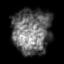
\includegraphics[width=0.2\textwidth]{Emd_8647_proj1.jpg}
\captionsetup{justification=centering}
\caption{EMD-8647t}
\end{subfigure} 
\begin{subfigure}{1\textwidth}
\centering
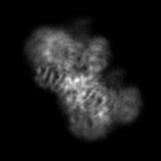
\includegraphics[width=0.2\textwidth]{Emd_4138_proj_1.jpg}
\captionsetup{justification=centering}
\caption{EMD-4138}
\end{subfigure}
\label{fig:emd_projection}
\end{figure}

\begin{figure}[H]
\centering
\begin{subfigure}{.5\textwidth}
\centering
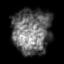
\includegraphics[width=0.8\linewidth]{Emd_8647_proj1.jpg}
\captionsetup{justification=centering}
\caption{ T20S-Proteasome }
\end{subfigure} 
\begin{subfigure}{.48\textwidth}
\centering
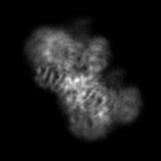
\includegraphics[width=0.8\linewidth]{Emd_4138_proj_1.jpg}
\captionsetup{justification=centering}
\caption{ 80S-Ribosome }
\end{subfigure}
\caption{Negative Sample (Dimension 216x216)}
\label{fig:Negative-Projection}
\end{figure}



\begin{figure}[H]
\centering

\begin{subfigure}{.3\textwidth}
\centering
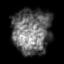
\includegraphics[width=0.8\linewidth]{Emd_8647_proj1.jpg}
\captionsetup{justification=centering}
\caption{ Noise 0\% }
\end{subfigure} 
\begin{subfigure}{.27\textwidth}
\centering
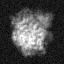
\includegraphics[width=0.8\linewidth]{Emd_8647_proj1_noise_10.jpg}
\captionsetup{justification=centering}
\caption{ Noise 10\%}
\end{subfigure}
\begin{subfigure}{.28\textwidth}
\centering
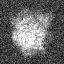
\includegraphics[width=0.8\linewidth]{Emd_8647_proj1_noise_30.jpg}
\captionsetup{justification=centering}
\caption{ Noise 30\%}
\end{subfigure}

\begin{subfigure}{.3\textwidth}
\centering
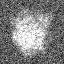
\includegraphics[width=0.8\linewidth]{Emd_8647_proj1_noise_50.jpg}
\captionsetup{justification=centering}
\caption{ Noise 50\% }
\end{subfigure} 
\begin{subfigure}{.27\textwidth}
\centering
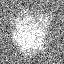
\includegraphics[width=0.8\linewidth]{Emd_8647_proj1_noise_80.jpg}
\captionsetup{justification=centering}
\caption{ Noise 80\%}
\end{subfigure}
\begin{subfigure}{.28\textwidth}
\centering
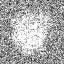
\includegraphics[width=0.8\linewidth]{Emd_8647_proj1_noise_100.jpg}
\captionsetup{justification=centering}
\caption{ Noise 100\%}
\end{subfigure}
\caption{EMD-8647 Projections}
\label{fig:EMD-8647 Projections: Noisy}
\end{figure}





\begin{figure}[H]
\centering

\begin{subfigure}{1\textwidth}
\centering
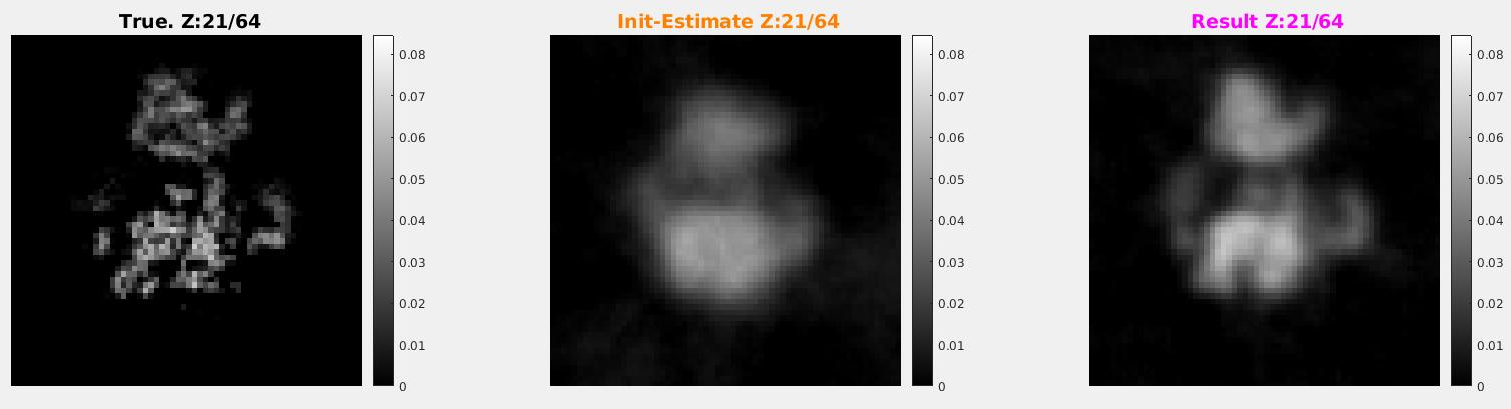
\includegraphics[width=1\linewidth]{emd_8647_result_1.png}
\captionsetup{justification=centering}
\caption{ Slice-21 }
\end{subfigure} 

\begin{subfigure}{1\textwidth}
\centering
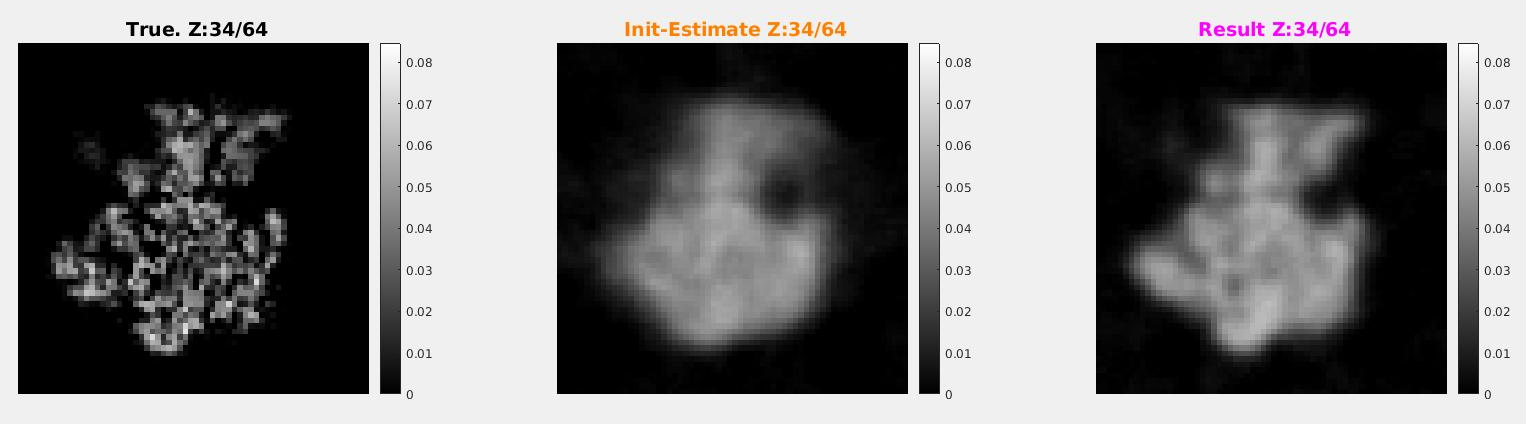
\includegraphics[width=1\linewidth]{emd_8647_result_2.png}
\captionsetup{justification=centering}
\caption{ Slice-34 }
\end{subfigure} 

\begin{subfigure}{1\textwidth}
\centering
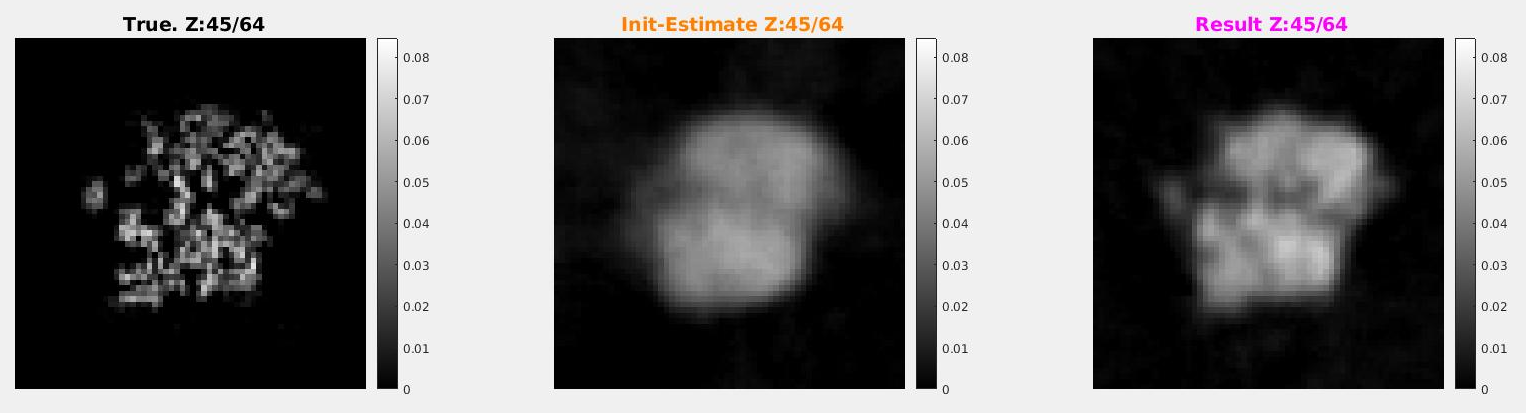
\includegraphics[width=1\linewidth]{emd_8647_result_3.png}
\captionsetup{justification=centering}
\caption{ Slice-45 }
\end{subfigure} 

\begin{subfigure}{1\textwidth}
\centering
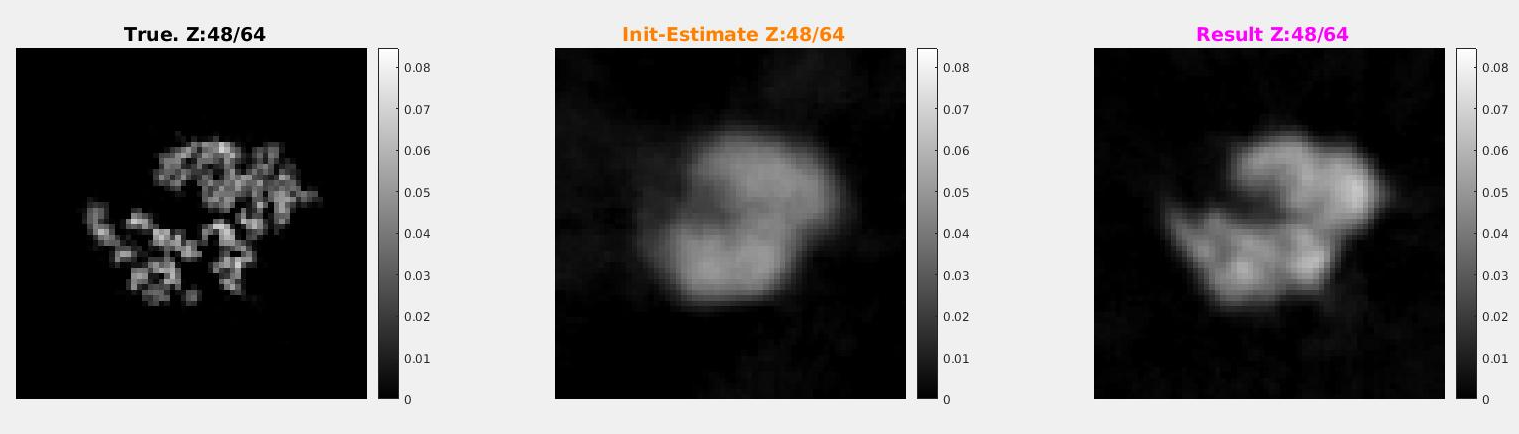
\includegraphics[width=1\linewidth]{emd_8647_result_4.png}
\captionsetup{justification=centering}
\caption{ Slice-48 }
\end{subfigure} 


\caption{EMD-8647 Reconstruction Result for noise level 100\%}
\label{fig:EMD-8647 Reconstruction: Result-noise 100}
\end{figure}





\begin{figure}[H]
\centering

\begin{subfigure}{1\textwidth}
\centering
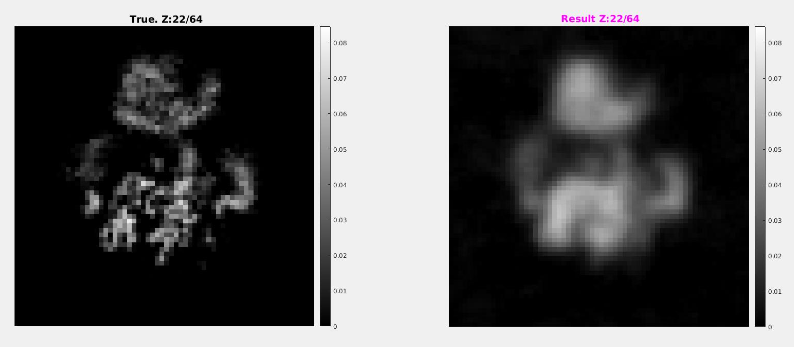
\includegraphics[width=1\linewidth]{emd_8647_result_sharp_1.png}
\captionsetup{justification=centering}
\caption{ Slice-21 }
\end{subfigure} 

\begin{subfigure}{1\textwidth}
\centering
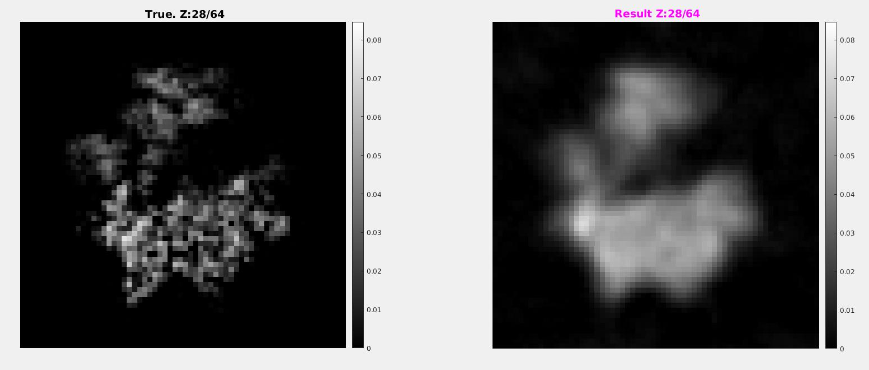
\includegraphics[width=1\linewidth]{emd_8647_result_sharp_2.png}
\captionsetup{justification=centering}
\caption{ Slice-34 }
\end{subfigure} 

\begin{subfigure}{1\textwidth}
\centering
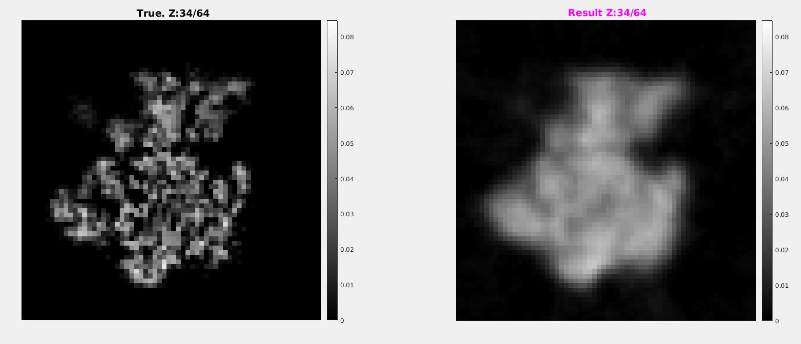
\includegraphics[width=1\linewidth]{emd_8647_result_sharp_3.png}
\captionsetup{justification=centering}
\caption{ Slice-45 }
\end{subfigure} 

\begin{subfigure}{1\textwidth}
\centering
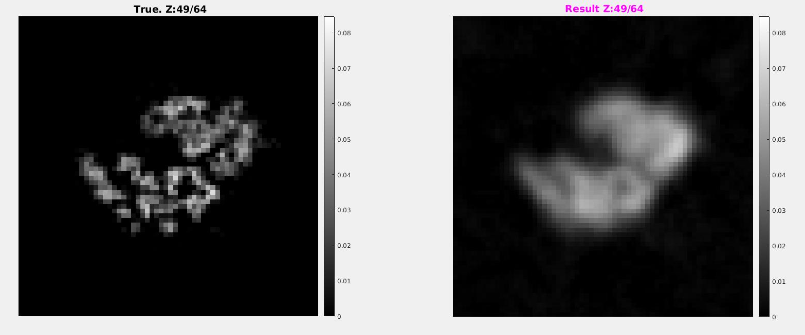
\includegraphics[width=1\linewidth]{emd_8647_result_sharp_4.png}
\captionsetup{justification=centering}
\caption{ Slice-48 }
\end{subfigure} 


\caption{EMD-8647 reconstruction result for noise level 100  \%}
\label{fig:EMD-8647 Reconstruction: Result-noise 100}
\end{figure}

\subfile{temp3}



\end{document}